\section{Introduction}
\paragraph{}
The Progressive Era was a time that saw many different people reacting to
unregulated laissez-faire capitalism, You could say that ``progressive''
means to try to use government to make things better for people.
While some people tried to fight for better conditions, fairer legislation,
improved working conditions, and quality of life. These people, or ``progressives''
could take the form of muckrakers who exposed the unjust of working and living
onditions, such as Jacob Riis, and Upton Sinclair. By total accident Theodore
Roosevelt became president in 1901. Corrupt Corporations thought they could
control him. They were gravely wrong, Roosevelt was the incorruptable hero
of the progressive Movement

\section{Taking on the Captains of Industry}
\paragraph{}
Theodore Roosevelt took the captains of industry head on. With such things as
antitrust prosecutions, and regulatory control. One example of his regulatory
control is pushing legislation to give the ICC (Interstate Commerce Comission)
the power to set railroad and shipping rates. Another progressive act was the
pre food, drug, and meat act, assuring quality control and regulation. When
Theodore Roosevelt was a New York Assemblyman he aided in the passing of a law
to prohibit the production of cigars in tenement houses, also exposing the
rampant bribery and corruption in the legislature caused by
``special interests'' and ``political machines''. To aid congress in decision
making regarding big bussiness Theodore Roosevelt established the ``Bureau
of Coporations'' during his presidency. In the eyes of Theodore Roosevelt,
taking on the captains of industry and ending corruption wasd doing nothing
more then following in the footsteps of people such as Geogre Washington,
Alexander Hamilton, and Abraham Lincoln.

\section{Theodore Roosevelt, Steward of Natural Resources}
\paragraph{}
Appointing himself ``Stweard of Natural Resources'', Theodore Roosevelt
started the conservation movement. A movement to perserve and protect
the nations' natural untouched landscapes. Roosevelt setup wildlife and
bird refuges, to perserve Americas' animals. Also appointing certain
locations as national landmarks, monuments, and historic areas, Such
as the grand canyon. Devil's Tower, El Morro, Lewis \& Clark Caverns, and
Lassen Peak are just a few of the Nation Monuments Theodore Roosevelt
established. From his experience in the Dakota Bandlands, Theodore Roosevelt
was inspired to preserve, and protect Americas' natural beauty.

\section{Theodore Roosevelt, and \textit{How the Other Half Lives}}
\paragraph{}
Reading \textit{How the Other Half Lives} By Jacob Riis, had a profound
effect on Theodore Roosevelts' drive for progressivism. In 1984 Roosevelt
met Jacob Riis, muckraker, and author of \textit{How the Other Half Lives}.
Often having Riis acompany him on police beats. ``When Roosevelt read [my]
book, he came\ldots{}No one ever helped as he did. For two years we were brothers
in (New York City's crime-ridden) Mulberry Street. When he left I had seen its
golden age\ldots{}''~\cite{jacobriis1901}.\\

\begin{wrapfigure}{r}{0.25\textwidth}
	\centering
	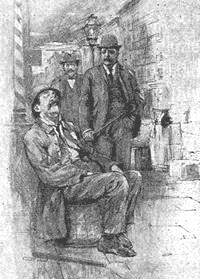
\includegraphics[width=0.25\textwidth]{beat.jpg}
\end{wrapfigure}

The illustration to the right is from Jacob Riis' autobiography.
\cite{jacobriis1901}
Reading Riis's book and meeting him, gave Roosevelt a greater understanding
into the life of the impoverished, and working class. This new found empathy
allowed Roosevelt to fully understand the evil that was caused by the
uncontroleld growth of industry.

\section{Conclusion}
The Golden era of reform brought many needed changes to the untame
viral spread of industry. Rampant reform stopped the choking control
that industry had over the government, and the people it represented.
Progressives left their mark on history and will never be forgotten.
Theodore Roosevelts' accidental presidency ended up being one of the
worst things for big business.

\newpage
\printbibliography{}
